\section{Intuition}
\subsection{Bottleneck Paths}
\label{section:subdividing-bottlenecks}
Before we reveal the algorithm for Network Diversion, we will first look at a curious little problem that we call \textsc{Shortest Bottleneck Path}:

\fbox{\parbox{0.94\textwidth}{\textsc{Shortest Bottleneck Path}\\
    \textbf{Input:} A graph $G$, two vertices $s,t \in V$, and a 'bottleneck' edge $b \in E$\\
    \textbf{Output:} the shortest $s$-$t$-path in $G$ that goes through the bottleneck $b$
}}

There is no obvious way to solve \textsc{Shortest Bottleneck Path}. One might attempt to find the shortest paths from $s$ to $from(b)$ and from $to(b)$ to $t$, but those two paths might overlap and reuse the same vertices, and therefore would their concatenation not necessarily be a path but just a walk instead.

\begin{figure}
    \centering
    \begin{subfigure}{.80\textwidth}
        \centering
        % 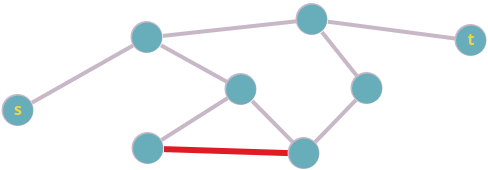
\includegraphics[width=6cm]{figures/bottleneck.png}
        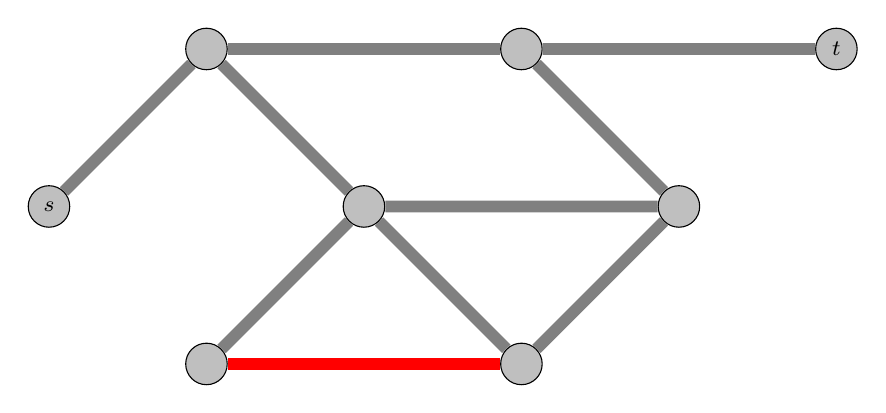
\begin{tikzpicture}
            \tikzstyle{every node}=[circle, fill=lightgray, draw=black, inner sep=2pt, minimum size=1.5em, font=\footnotesize, text=black]
            \tikzstyle{edge}=[gray, line width=1.5mm]
        
            \node (s) at (0,0) {$s$};
            \node (a) at (2,2) {};
            \node (b) at (4,0) {};
            \node (c) at (2,-2) {};
            \node (d) at (6,-2) {};
            \node (e) at (8,0) {};
            \node (f) at (6,2) {};
            \node (t) at (10,2) {$t$};
        
            \draw[edge] (s) -- (a) -- (b) -- (e);
            \draw[edge] (c) -- (b) -- (d) -- (e) -- (f) -- (t);
            \draw[edge] (a) -- (f);
        
            \tikzstyle{edge}=[red, line width=1.5mm]
            \draw[edge] (c) -- (d);
        \end{tikzpicture}
        \caption{An instance of \textsc{Shortest Bottleneck Path}, bottleneck marked in red.}
        \label{figure:bottleneck}
    \end{subfigure}\hfill%
    \begin{subfigure}{.80\textwidth}
        \centering
        % 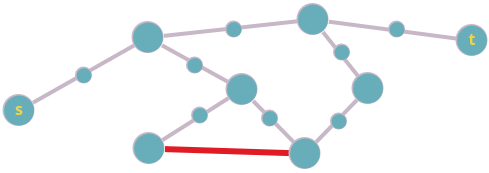
\includegraphics[width=6cm]{figures/subdivide-bottleneck.png}
        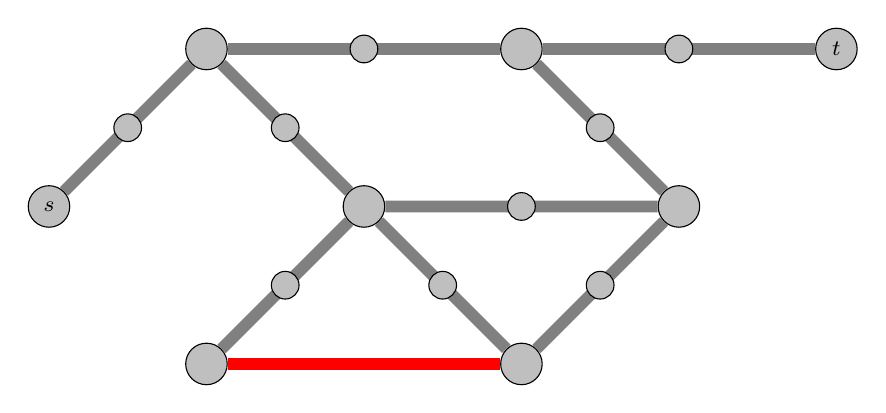
\begin{tikzpicture}
            \tikzstyle{every node}=[circle, fill=lightgray, draw=black, inner sep=2pt, minimum size=1.5em, font=\footnotesize, text=black]
            \tikzstyle{edge}=[gray, line width=1.5mm]
        
            \node (s) at (0,0) {$s$};
            \node (a) at (2,2) {};
            \node (b) at (4,0) {};
            \node (c) at (2,-2) {};
            \node (d) at (6,-2) {};
            \node (e) at (8,0) {};
            \node (f) at (6,2) {};
            \node (t) at (10,2) {$t$};
        
            \draw[edge] (s) -- (a) -- (b) -- (e);
            \draw[edge] (c) -- (b) -- (d) -- (e) -- (f) -- (t);
            \draw[edge] (a) -- (f);
        
            \tikzstyle{edge}=[red, line width=1.5mm]
            \draw[edge] (c) -- (d);

            \tikzstyle{every node}=[circle, fill=lightgray, draw=black, inner sep=2pt, minimum size=1em, font=\footnotesize, text=black]
            \node (sa) at (1,1) {};
            \node (af) at (4,2) {};
            \node (ab) at (3,1) {};
            \node (bc) at (3,-1) {};
            \node (bd) at (5,-1) {};
            \node (be) at (6,0) {};
            \node (de) at (7,-1) {};
            \node (ef) at (7,1) {};
            \node (ft) at (8,2) {};
        \end{tikzpicture}
        \caption{All edges except the bottleneck have been subdivided.}
        \label{figure:subdivided-bottleneck}
    \end{subfigure}%
    \caption{\textsc{Shortest Bottleneck Path} reduced to \textsc{Shortest Odd Path} by subdividing edges.}
    \label{figure:bottleneck-subdividing}
\end{figure}

Instead we create a new graph $H$, by subdividing all edges in $G$ \emph{except} $b$, like seen in figure \ref{figure:bottleneck-subdividing}. The key point to see here is that any odd $s$-$t$-path in $H$ must necessarily go through the bottleneck, otherwise it would not be odd. We can visualize it by 'stepping through' the edges in $H$. If we start on our right leg, then in the beginning every time we reach a vertex that is also in $G$, we reach it by stepping on our left leg. That continues until we use the bottleneck edge, and from then on we step on all vertices from $G$ using our right leg. If we require that we must end at $t$ on our right leg, then the path must be odd, and any odd path must go through the bottleneck. Therefore we can simply run our Shortest Odd Path algorithm on $H$, and if such a path exists we can reverse the subdivision of the edges in the path and the result is the Shortest Bottleneck Path in $G$.

If we extend the problem to have multiple bottleneck edges, and we have to go through all of them, then our idea will not work. \todo{Fact check}That is good, because otherwise we would have solved the Traveling Salesman Problem in polynomial time and complexity theory as we know it would break down.
The problem is that we have no way of knowing whether we have used the marked edges 1, or 3, or 5, etc. times, because in all of them we hit vertices from $G$ using our right leg. We can, however, use this idea to find paths that use a certain set of edges an odd amount of times. As it turns out, that is exactly what we need to solve Network Diversion.


\subsection{From a dual cycle to a real diversion}
\todo{seriøst bedre tittel enn dette}
Remember, we want to find the minimum minimal $s$-$t$-cut that includes $d$. \todo{Trenger bedre intro} We will start with a cycle in the dual graph and add restrictions until we have what we want.

Let us start off by finding a path in the dual graph, from and to the regions to the left and right of $d$, Then, we add $d^\star$ to the path, to make it a cycle. As explained in Fact \ref{fact:dual-cycle-is-real-cut}, this simple cycle in the dual graph must correspond to a cut in the original graph. Since it both includes $d^\star$ and does not repeat any other edges or vertices, it corresponds to a minimal cut that uses $d$.

This cut is not necessarily an $s$-$t$-cut in $G$. To be such a cut, the cycle needs to go 'around' either $s$ or $t$, but not both. Otherwise $s$ and $t$ would end up in the same component. There is no obvious way to force that, but we will show an as for now unpublished trick. Find first any $s$-$t$-path in $G$ that does not use the diversion edge $d$. Then subdivide all the edges in the dual graph, except those that cross edges in that $s$-$t$-path. If we now find an \emph{odd} path from and to the left and right regions of $d$, then this must be a path that crosses the $s$-$t$-path an odd number of times. Therefore, the $s$-$t$-path must have exactly one endpoint on the 'inside' of the cycle, and the other on the 'outside'. That means it cuts off $s$ from $t$, and is therefore an $s$-$t$-cut of $G$. 

If this odd path is also the shortest odd path, then the corresponding cut is the minimum minimal $s$-$t$-cut of $G$ that includes $d$, and the solution to this instance of \textsc{Network Diversion}.

\todo[inline]{more intuition for ND}